\section{Procédés de fabrication des MID}
Il existe actuellement 2 méthodes de production de \textsc{mid} sur le marché :
le \emph{Laser Direct Structuring} et le \emph{Two-shot molding}. Le premier est
de loin le plus répandu (environ 80\% du marché selon \cite{mid-2011}), car moins
cher et plus adapté aux petites séries, tandis que le second est utilisé lorsque
la géométrie de la pièce ne permet pas l'usage du \textsc{lds}.

\subsection{Laser Direct Structuring}
\begin{figure}[h]
    \begin{center}
        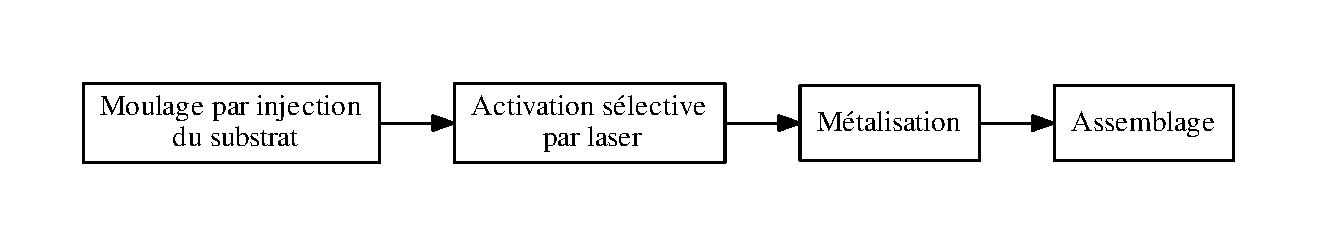
\includegraphics[width=\textwidth]{lds_process}
        \caption{Vue d'ensemble du processus \emph{Laser Direct Structuring}}\label{fig:lds-process}
    \end{center}
\end{figure}
